\originalsection{附录 F: 未过滤数据集结果}\paperlabel{F}{chive-app:allruns}
本附录展示两个主要结果不是B.3过滤产生的假象: 激活工具相对仅记录无增益, 反事实预测训练能泛化. 在完全未过滤主张上重跑两评价.

\textbf{未过滤集.} 正文三过滤是机制具体性$\ge3$、可重复、单因素. 具体性最大, 删除三分之一至三分之二主张. 因而试移除全部过滤, Gemma从1294到4433, Qwen8B从1497到4041, Qwen397B从1076到3972. 真标签47--53\%, 近乎平衡, 报无阈值AUROC.

\textbf{工具在未过滤集也无增益}（图 \ref{chive-fig:unfiltered_tools}）. 完整Gemma集仍无工具超过基线. 绝对表现比过滤低几个百分点, 因更多机制模糊、不易预测的反事实.
\begin{figure}[ht]\centering
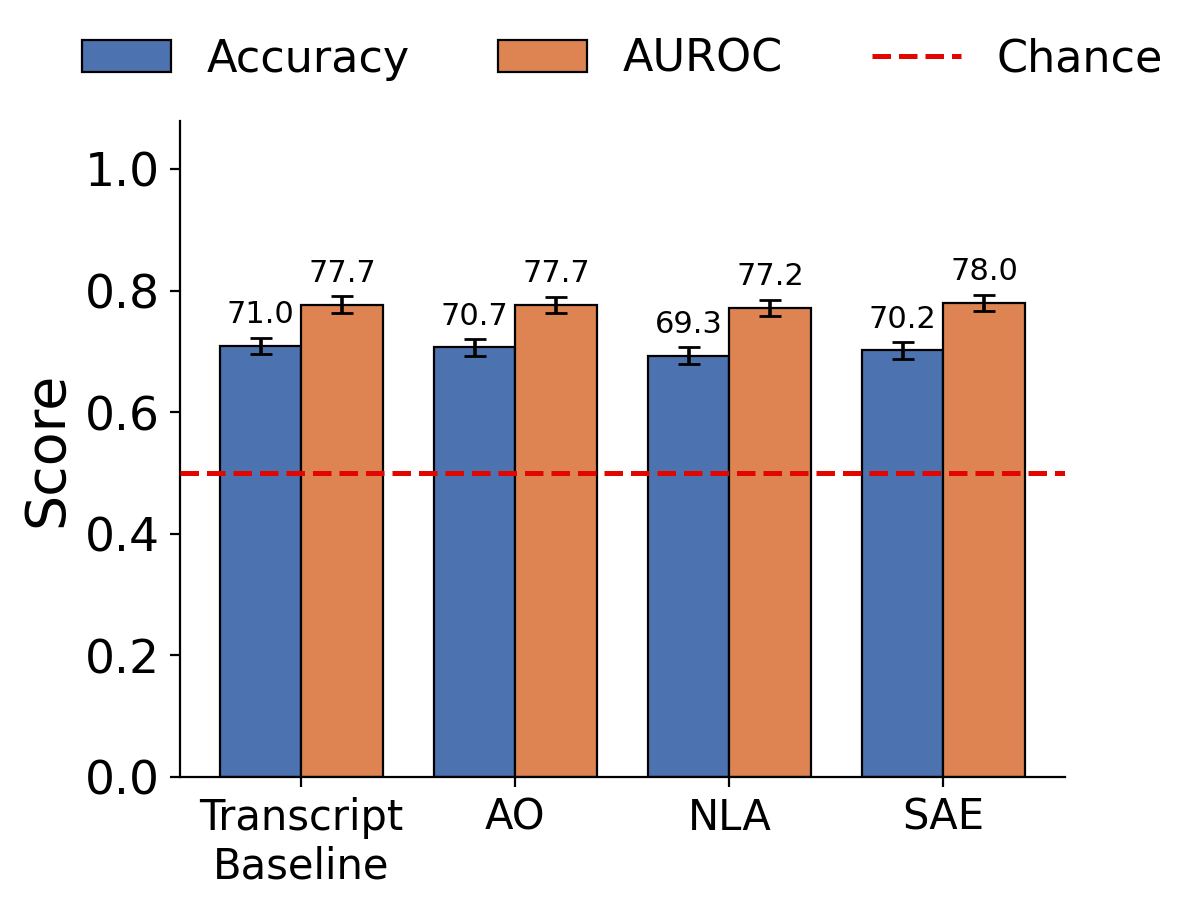
\includegraphics[width=.6\linewidth]{../papers/translations/chive/figures/gemma_unfiltered_overall_score.png}
\caption{未过滤集工具仍无增益, Gemma-3-27B-IT, $n=4433$. 图例: Transcript only＝仅记录, AO/NLA/SAE分别为激活预言机/自然语言自编码器/稀疏自编码器; AUROC为ROC面积.}\label{chive-fig:unfiltered_tools}
\end{figure}

\textbf{未过滤时训练反事实模型略超Opus参照}（图 \ref{chive-fig:unfiltered_trained}）. 过滤集达到参照, 相对Opus配对$\Delta$AUROC: Qwen8B为$-.001$[$-.021,+.020$], Qwen397B为$+.013$[$-.009,+.035$]. 未过滤略高: 分别$+.015$[$+.002,+.027$]、$+.033$[$+.021,+.044$]. 改善集中在具体性过滤删掉的低具体性主张. 具体性1--2上, 训练8B AUROC .848, Opus .822; 训练397B .852, Opus .811. 换言之, 行为机制模糊处训练最有帮助.
\begin{figure}[ht]\centering
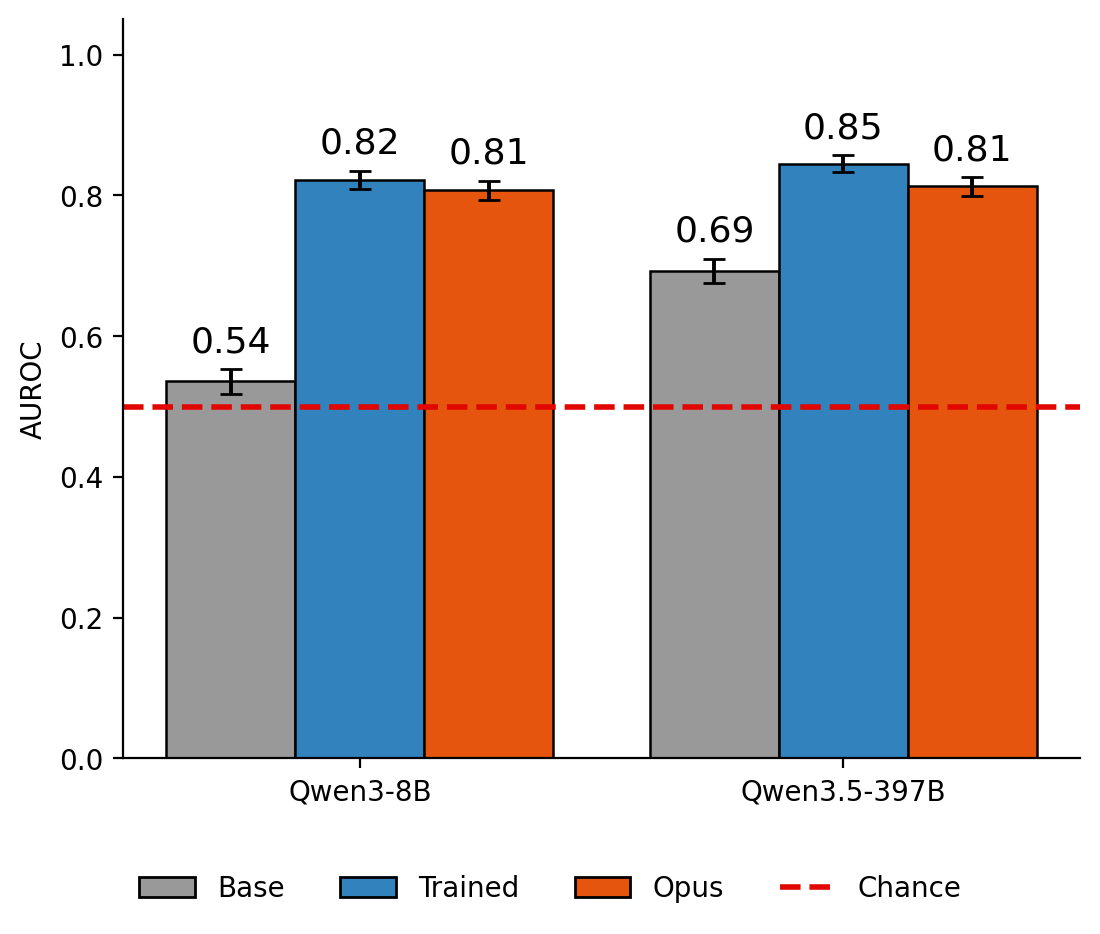
\includegraphics[width=.6\linewidth]{../papers/translations/chive/figures/unfiltered_direct_cf_auroc.png}
\caption{未过滤时训练反事实模型略超Opus参照. WildChat, Qwen3-8B $n=4041$, Qwen3.5-397B $n=3972$. 图例: Base＝基础, Trained＝训练, Opus reference＝参照; 纵轴为AUROC.}\label{chive-fig:unfiltered_trained}
\end{figure}

\originalsection{附录 G: 真实场景中不忠实的思维链}\paperlabel{G}{chive-app:cot}
忠实性文献多在暗示设置取得真值, 植入一种已知线索、测一种预定义行为. 真实场景也已记录不忠实思维链: Arcuschin等通过模板提示的逻辑不一致, 展示前沿模型在未植入线索时产生不忠实推理\cite{chive-arcuschin2026chainofthoughtreasoningwildfaithful}, 如同时对“$X>Y$?”和“$Y>X$?”答Yes. 本流程用于推理模型能得到更多多样案例. 除传统不忠实外, 还发现思维链对决策重要部分不置一词等异常行为. 此处报告定性例子, 系统研究留作后续.

用相同WildChat提示, 在Qwen3-8B启用推理、思考预算1024token重跑完整流程; 对生成主张重跑可解释性评价, 质量切片同正文. 还发布Qwen3.5-397B-A17B推理调查集, 未作分析, 供未来工作.

\textbf{推理资料上工具零增益不变.} 无工具胜仅记录（图 \ref{chive-fig:cot_interp}）. 总体比非思考高, 仅记录AUROC .87对.81, 可能因可见推理帮助基线. 高分不表示饱和, 困难子集也相同: 限定基线不确定、预测概率$[.25,.75]$的主张, 保留65\%即$n=933$, 基线AUROC降.78.
\begin{figure}[ht]\centering
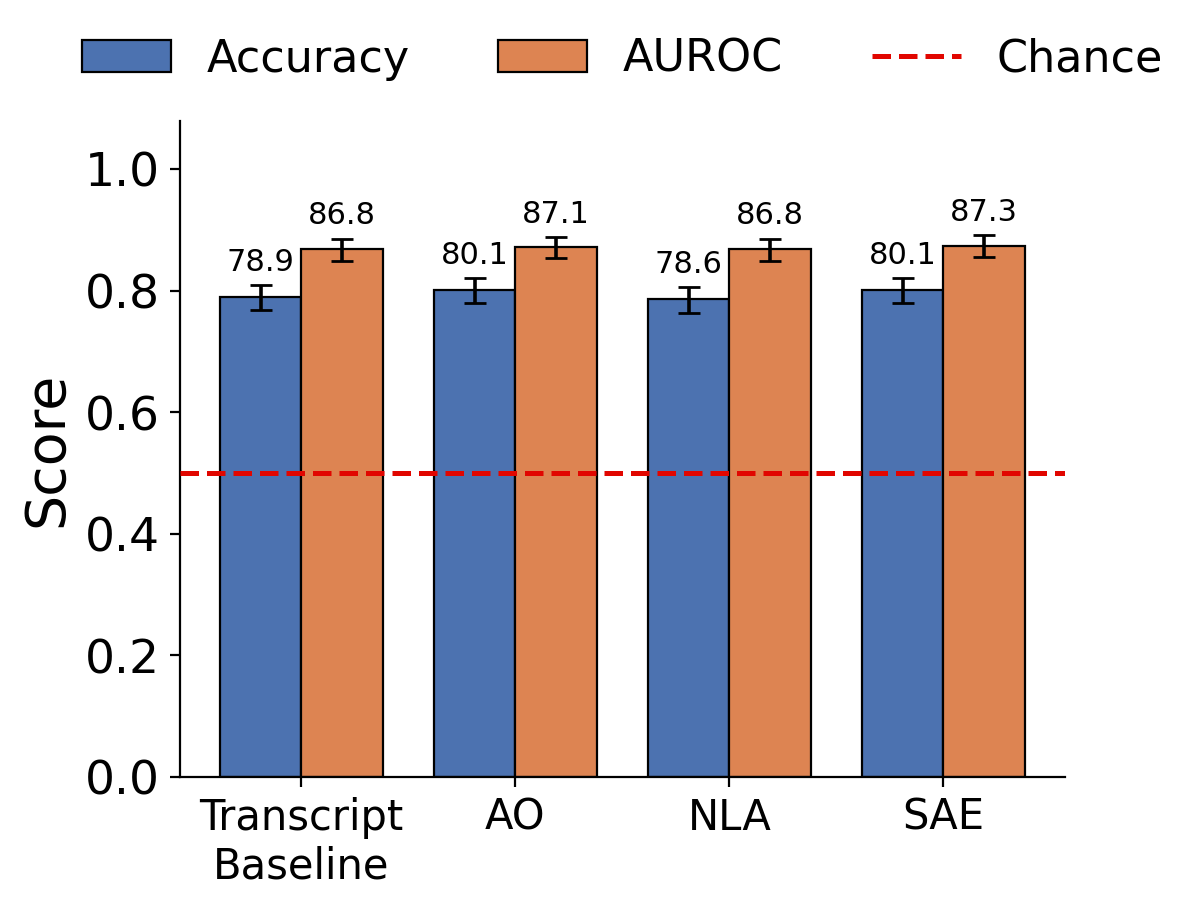
\includegraphics[width=.85\linewidth]{../papers/translations/chive/figures/thinking_overall_score.png}
\caption{推理模式资料上工具也无增益. 第 \ref{chive-sec:interp_eval} 节评价在启用推理的Qwen3-8B重跑. 无工具胜仅记录, 在包含明确推理记录的对话中复现非思考结果. 图例: Transcript only＝仅记录, AO/NLA/SAE为三个工具, Score＝成绩, Accuracy＝准确率, AUROC＝ROC面积, Chance＝随机水平.}\label{chive-fig:cot_interp}
\end{figure}
给出评价集两个定性例子.

\textbf{例: 节目选择遗漏的原因.} 从14节目名单选两个写短故事, 模型每回答都选《Phineas and Ferb》（《飞哥与小佛》）. 思维链归因知名度:“Phineas and Ferb was a big hit, so that's a good one”（很火, 所以好选择）. 反事实表明最重要原因是名单位置, 而非知名度: 放首位30/30选择, 移末位降4/30.

\textbf{例: 无法从思维链预测的行动.} 流程还发现许多传统上不归为不忠实的行为: 模型没断言错误原因, 但行动仍不能由推理预测. 一个提示要求架空历史时间线, 用户称Woodrow Wilson（伍德罗·威尔逊）为“the world's first fascist dictator”（世界首位法西斯独裁者）. 模型29/30回答写真实、寻求和平的Wilson. 推理计划地缘政治, 但27/30完全不提如何描写Wilson, 余三次把历史中立性当事实,“Wilson is neutral, trying to keep US out”（Wilson中立, 试图不让美国参战）, 不提提示相反. 换成虚构名字后和平描写仅3/30. 真实Wilson知识压过用户明确要求, 推理中却不可见.
